\chapter{Results}

The results of my research have been at several conferences.
The following sections include these publications.

%The following publications are included in this chapter:
%
%\begin{enumerate}
%	%\item Filip Bártek and Martin Suda. Learning Precedences from Simple Symbol Features. \Gls{paar} 7, 2020. \cite{DBLP:conf/cade/Bartek020}
%	\item Filip Bártek and Martin Suda. Neural Precedence Recommender. \Gls{cade} 28, 2021. \cite{DBLP:conf/cade/Bartek021}
%	\item Filip Bártek and Martin Suda. How much should this symbol weigh? A \acrshort{gnn}-Advised Clause Selection \cite{DBLP:conf/lpar/Bartek023}
%	\item Filip Bártek, Karel Chvalovský, and Martin Suda. Regularization in Spider-Style Strategy Discovery and Schedule Construction. \Gls{ijcar}, 2024 (accepted). \cite{bartek2024regularization}
%\end{enumerate}

\section{Neural Precedence Recommender}
\label{sec:results:npr}

Filip Bártek and Martin Suda. Learning Precedences from Simple Symbol Features. \Gls{paar} 7, 2020. \cite{DBLP:conf/cade/Bartek020}

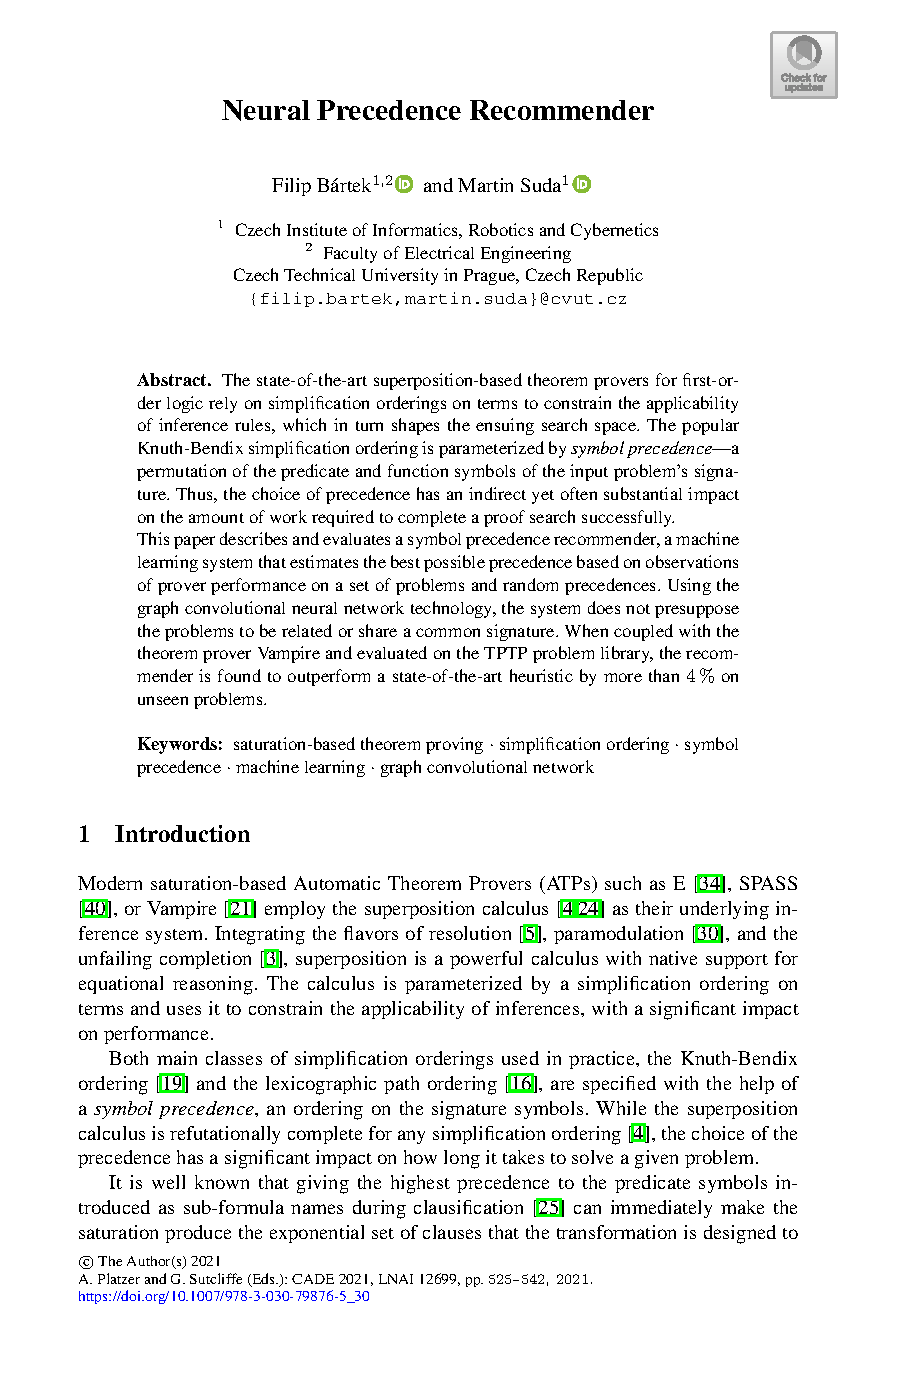
\includepdf[pages=-]{publications/Neural Precedence Recommender.pdf}

\section{A GNN-Advised Clause Selection}
\label{sec:results:gnn}

Filip Bártek and Martin Suda. How much should this symbol weigh? A \acrshort{gnn}-Advised Clause Selection \cite{DBLP:conf/lpar/Bartek023}

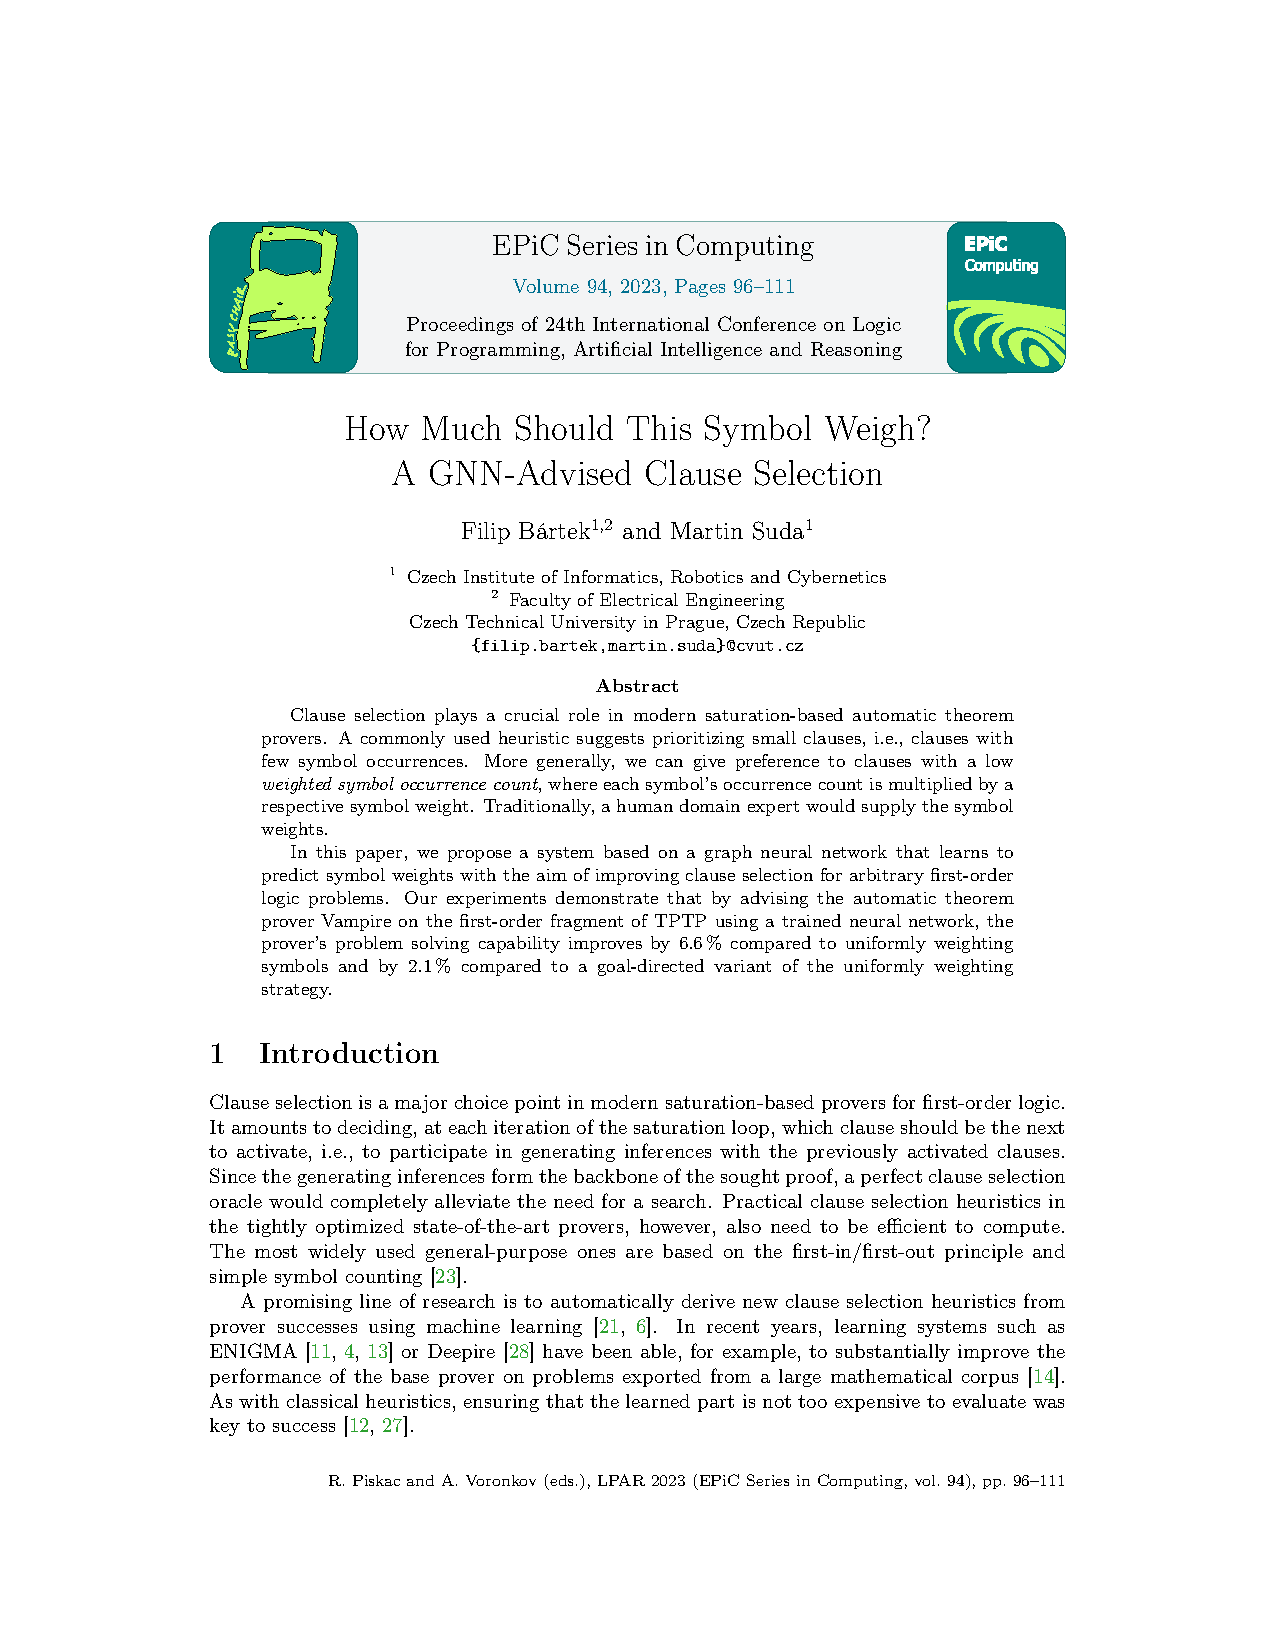
\includepdf[pages=-]{publications/How_Much_Should_This_Symbol_Weigh_A_GNN-Advised_Clause_Selection.pdf}

\section{Regularization}
\label{sec:results:regularization}

Filip Bártek, Karel Chvalovský, and Martin Suda. Regularization in Spider-Style Strategy Discovery and Schedule Construction. \Gls{ijcar}, 2024 (accepted). \cite{bartek2024regularization}

% TODO: Replace by the final version and link to the arXiv version with appendix.
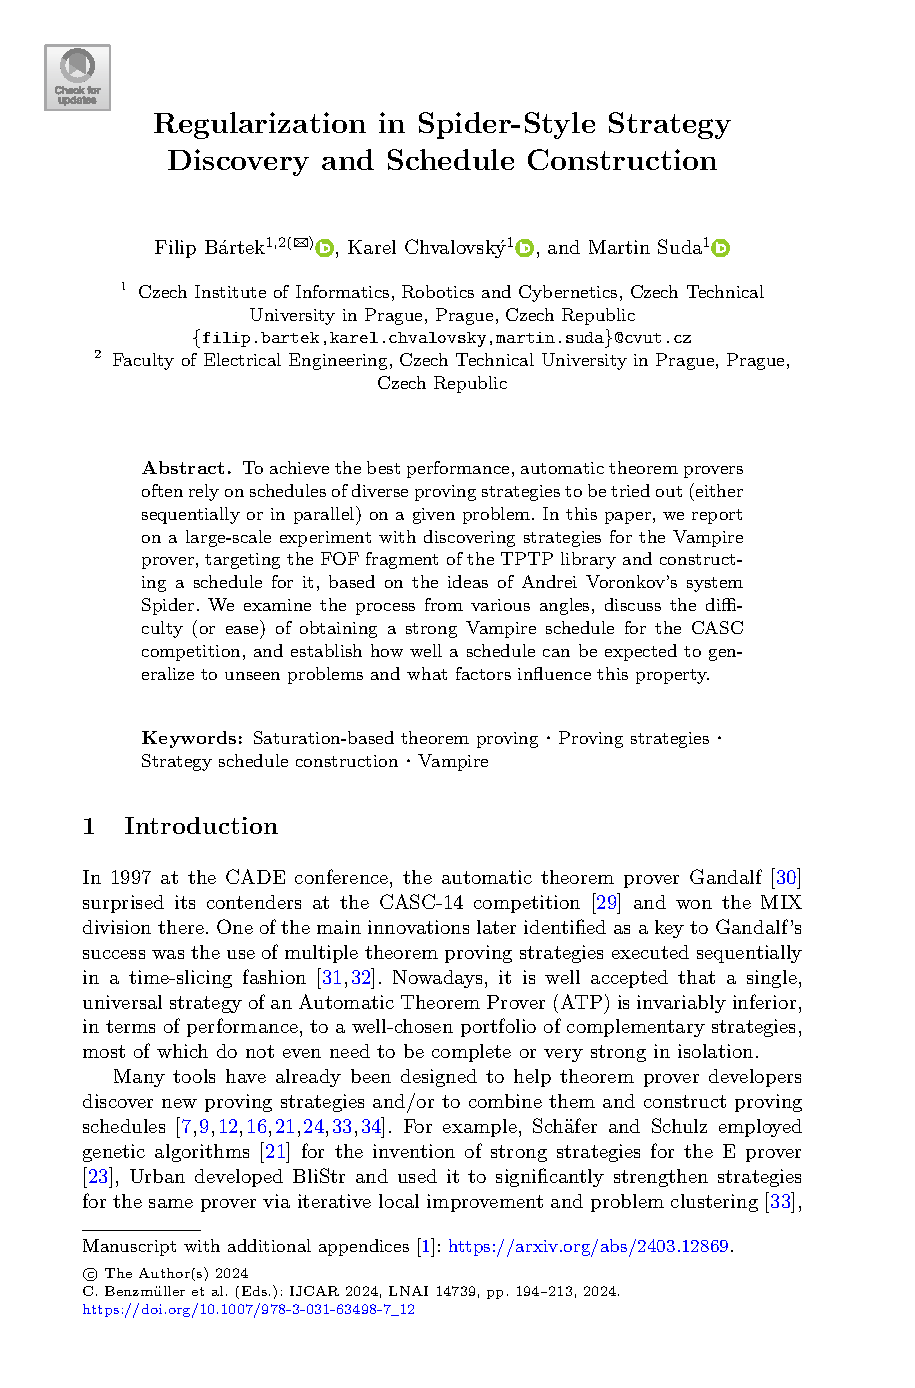
\includepdf[pages=-]{publications/regularization.pdf}
